\documentclass[10pt,handout]{beamer}
\usetheme[
%%% options passed to the outer theme
%    hidetitle,           % hide the (short) title in the sidebar
%    hideauthor,          % hide the (short) author in the sidebar
%    hideinstitute,       % hide the (short) institute in the bottom of the sidebar
%    shownavsym,          % show the navigation symbols
%    width=2cm,           % width of the sidebar (default is 2 cm)
%    hideothersubsections,% hide all subsections but the subsections in the current section
%    hideallsubsections,  % hide all subsections
%    right                % right of left position of sidebar (default is right)
  ]{Aalborg}

\definecolor{aaublue}{RGB}{33,26,82}
\definecolor{aaugrey}{RGB}{84,97,110}

% If you want to change the colors of the various elements in the theme, edit and uncomment the following lines
% Change the bar and sidebar colors:
\setbeamercolor{Aalborg}{fg=aaublue!10,bg=aaugrey!60}
%\setbeamercolor{sidebar}{bg=blue!74}
% Change the color of the structural elements:
\setbeamercolor{structure}{fg=aaublue}
 \setbeamercolor{subtitle}{fg=aaugrey}
% Change the frame title text color:
\setbeamercolor{frametitle}{fg=aaublue}
% Change the normal text color background:
%\setbeamercolor{normal text}{bg=aaugrey!10}
% ... and you can of course change a lot more - see the beamer user manual.
\usebackgroundtemplate{
\includegraphics[width=\paperwidth]{img/background}}

\usepackage[utf8]{inputenc}
\usepackage[english]{babel}
\usepackage[T1]{fontenc}
\usepackage{subfig} % Vi kan nu bruge \subfloat
\usepackage{soul} % use this (many fancier options)
\DeclareUnicodeCharacter{00A0}{~} % Fixes the "! Package inputenc Error: Unicode char \u8:  not set up for use with LaTeX."
% ... or whatever. Note that the encoding and the font should match. If T1
% does not look nice, try deleting the line with the fontenc.
\usepackage{lmodern} %optional

\usepackage[svgpath=img/]{svg} % Smart inclusion of SVG figures with \includesvg

% colored hyperlinks
\newcommand{\chref}[2]{%
  \href{#1}{{\usebeamercolor[bg]{Aalborg}#2}}
}

\title[]% optional, use only with long paper titles
{\includegraphics[width=5cm]{../thesis/frontmatter/aauship}\\ Formation Control of\\Autonomous Surface Vehicles for\\Surveying Purposes}

%\subtitle[v.\ 0.1.1] %optional
%{v.\ 0.1.1}

\author[14gr1034]{% optionally input the group number, use only with lots of authors
  Nick Østergaard \and Jeppe Dam\\
  {{\tt \{nickoe,jeppedam\}@es.aau.dk}}
}
% - Give the names in the same order as they appear in the paper.
% - Use the \inst{?} command only if the authors have different
%   affiliation. See the beamer manual for an example

%specify some optional logos
\pgfdeclareimage[height=1.2cm]{mainlogo}{aau_logo.pdf} % placed in the upper left/right corner
\logo{\pgfuseimage{mainlogo}}

\pgfdeclareimage[height=0.75cm]{logo2}{tu-logo} % placed in the lower left/right corner if the \pgfuseimage{logo2} command is uncommented in the \institute command below

\institute[
%  {\pgfuseimage{logo2}}\\ %insert a company or department logo
  Dept.\ of Electronic Systems,\\
  Aalborg University,\\
  Denmark
] % optional - is placed in the bottom of the sidebar on every slide
{%
  Department of Electronic Systems,\\
  Aalborg University,\\
  Denmark
  
  %there must be an empty line above this line - otherwise some unwanted space is added between the university and the country (I do not know why;( )
}
\date{\today}

\begin{document}
\setbeamertemplate{caption}{\raggedright\insertcaption\par}
% the titlepage
\begin{frame}[plain] % the plain option removes the sidebar and header from the title page
  \titlepage
\end{frame}
%%%%%%%%%%%%%%%%

% TOC
\begin{frame}{Agenda}{}
\tableofcontents
\end{frame}
%%%%%%%%%%%%%%%%
\section{Introduction}
\begin{frame}{Introduction}{Motivation}
  \begin{itemize}
    \item Port of Aalborg wants to be an intelligent harbour
    \item Always updated bathymetry data for an ``automatic pilot''
    \item Currently mapped with a manned boat
    \begin{itemize}
      \item Previously using a single beam echo sounder
      \item Now using a multi beam sonar
    \end{itemize}
    \item Bathymetry data is currently updated every three month to every three years approximately
    \item Can use autonomous vehicles to verify validity of old data
    \item A fleet of ``cheap'' autonomous vehicles could update the map in areas which do not require higher resolution.
  \end{itemize}
\end{frame}

\begin{frame}{Introduction}{Motivation}
  \begin{figure}
	  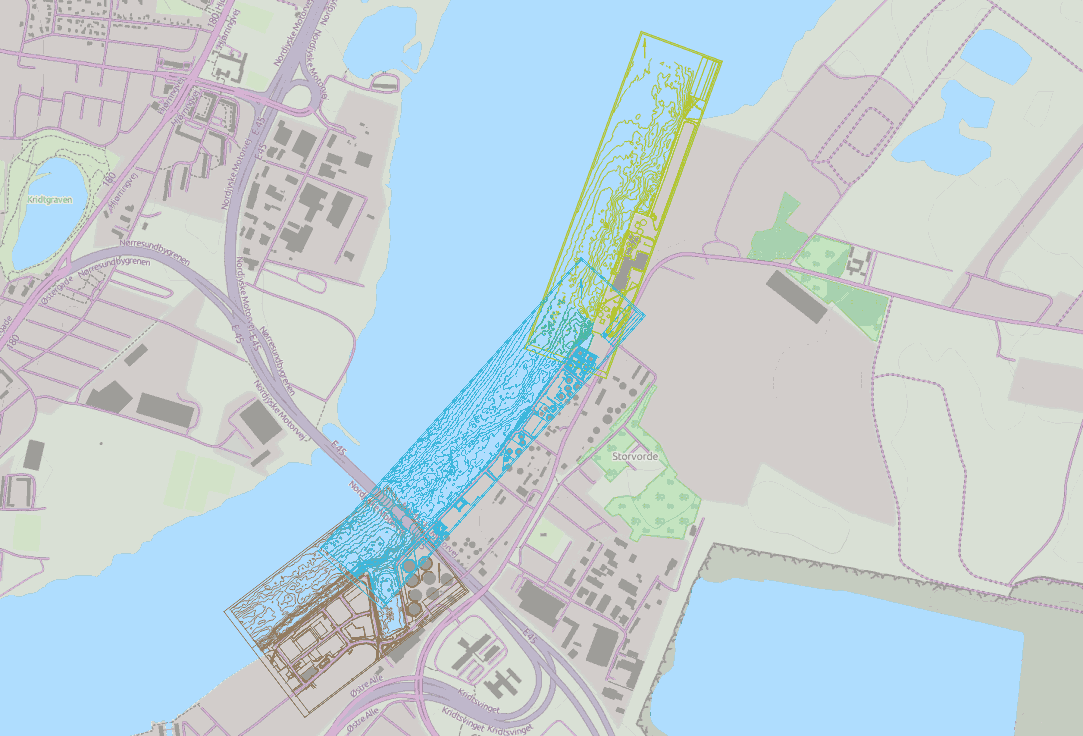
\includegraphics[width=\textwidth]{../thesis/fig/use-case-data}
	  \caption{\scriptsize Area of the harbour at Aalborg Portland, provided as sample
	  data from Aalborg Havn. Background map data CC BY-SA OpenStreetMap.}
  \end{figure}
\end{frame}

\begin{frame}{Introduction}{The Mission}
\begin{itemize}
\item Use Autonomous Surface Vessels (ASVs) for mapping with a single beam sonar
\item Control the ASVs with some formation control
\item Why is formation control beneficial in the context?
\begin{itemize}
\item Single beam / Multi beam
\item Faster
\item Easier detection
\item Followers to a main leader, offset to shallow water
\end{itemize}
\end{itemize}
\end{frame}

\begin{frame}{Introduction}{Concept Art}
\begin{figure}
  \centering
  \subfloat[One ship\label{fig:concept-art1}]{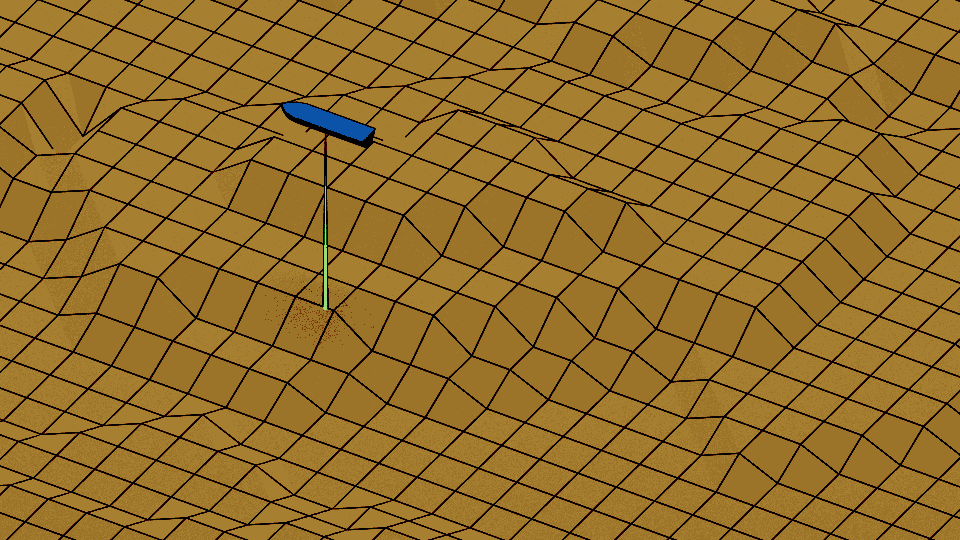
\includegraphics[width=0.48\textwidth]{../thesis/fig/conseptart-single}}
  \ % One forced space to seperate figures
  \subfloat[Thee ships\label{fig:concept-art3}]{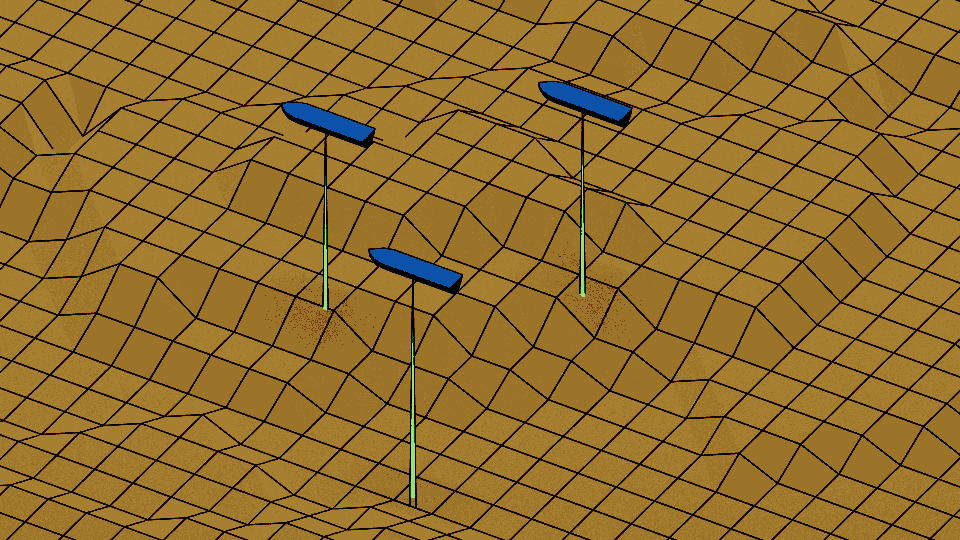
\includegraphics[width=0.48\textwidth]{../thesis/fig/conseptart-formation}}
  \caption{Comparison of two ways to cover an area with single beam ships}
  \label{fig:concept-art}
\end{figure}
\end{frame}

%\begin{frame}{Introduction}{1st Half Goals}
%Development of a single working testing platform
%  \begin{itemize}
%  \item Research of formation control paradigms
%  \item Decide feasibility for using ROS as the software platform
%  \item Subsystem test of the ship system, manual control
%  \item Modelling of the ship
%  \item Design and implementation of a state estimator
%  \item Creation of a simulation environment (Matlab and ROS)
%  \item \textit{Testing of autonomous control for a single ship}
%  \item \textit{Further research for the formation control task}
%  \end{itemize}
%\end{frame}


%%%%%%%%%%%%%%%%
\section{System Design}
\begin{frame}{System Design}{AAUSHIP.01}
\begin{itemize}
  \item The ship is designed as a non-planing deplacement craft (eg. like freight ships)
  \item Developed using rapid prototyping techniques
  \item Developed in Rhinoceros using lofting techniques
  \item Printed on a 3D printer
  \item Examined and the process iterated
  \item Vacuumformed by DD-plast in Randers and assembled at Aalborg University
\end{itemize}
\begin{center}
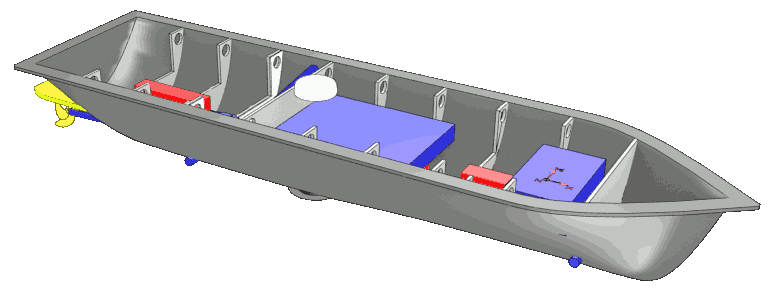
\includegraphics[width=0.5\textwidth]{img/blender-render}
\end{center}
\end{frame}

\begin{frame}{System Design}{Hardware}
\begin{itemize}
  \item Fitted with 2 brushless motors
  \item Fitted with 6 x 3200mAh batteries (results in a mission time of around 5 hours).
  \item 2 counter rotating 40mm propellers
  \item Inertial Measurement Unit
  \item Global Positioning System
  \item An ISM 20mW 19.2 kbps radio link 
  \item Microcontroller connects the ship electronics to the main computer (LLI)
  \item Netbook computer with ROS (HLI)
  \item Retrofitted with a hydrofoil to reduce the wake and pitch of the ship
\end{itemize}
\end{frame}

\begin{frame}{System Design}{Overview}
Modelling
\begin{itemize}
% <Describe what should be modelled, why 5DOF, parmeter estimation...>
\item What should be modelled?
\item How many states
\item Parameter estimation
\end{itemize}

Estimaiton
\begin{itemize}
% <KF and AHRS filters>
\item KF
\item AHRS
\end{itemize}

Simulation
\begin{itemize}
% <Simulation to model verification>
\item Simulation model in Matlab and ROS for office testing
\end{itemize}

Implementation with ROS
\begin{itemize}
\item ROS is modular, these are called nodes
\end{itemize}
\end{frame}

\begin{frame}{System Design}{ROS}
  \begin{figure}
    {\tiny \includesvg[width=\textwidth]{ros_aauship_closed_loop_single_beamer}}
	  \caption{\scriptsize The current ROS node and topic diagram, showing the elements that are implemented in black. Gray is to make it more user friendly.}
  \end{figure}
\end{frame}

%%%%%%%%%%%%%%%%
\section{Modelling}
\begin{frame}{Modelling}{Model}
  \begin{itemize}
    \item Using the linear ship model by Thor I. Fossen
    \item Extended with nonlinear calculations, like the trajectory calculation
    \item Saturation of inputs
    \item Thrust allocation included in the control node
  \end{itemize}
\end{frame}

\begin{frame}{Modelling}{Estimation with cheap GPS (low rate, low	resolution)}
  \begin{figure}
    {\tiny \includesvg[width=\textwidth]{intermediate-sensor-calculations-block}}
	  \caption{\scriptsize Block diagram of the combined AHRS and KF
		estimator. Implemented with cheap GPS only.}
  \end{figure}
\end{frame}

\begin{frame}{Modelling}{Estimation with expensive GPS (RTK)}
  \begin{figure}
    {\tiny \includesvg[width=\textwidth]{intermediate-sensor-calculations-block-rtk}}
    \caption{\scriptsize Block diagram of the combined AHRS and KF
		estimator. Implemented with RTK GPS only.}
  \end{figure}
\end{frame}

%%%%%%%%%%%%%%%%
\section{Simulation and Verificaiton}
%\begin{frame}{Simulation and Verificaiton}{Kalman Filter}
%  \begin{itemize}
%    \item Tuning of the KF
%    \item Tuning of the AHRS
%    \item Comparison and choice of heading estimate
%  \end{itemize}
%\end{frame}

%\begin{frame}{Simulation and Verificaiton}{Kalman Filter}
%Acceleration tuning
%  \begin{figure}
%    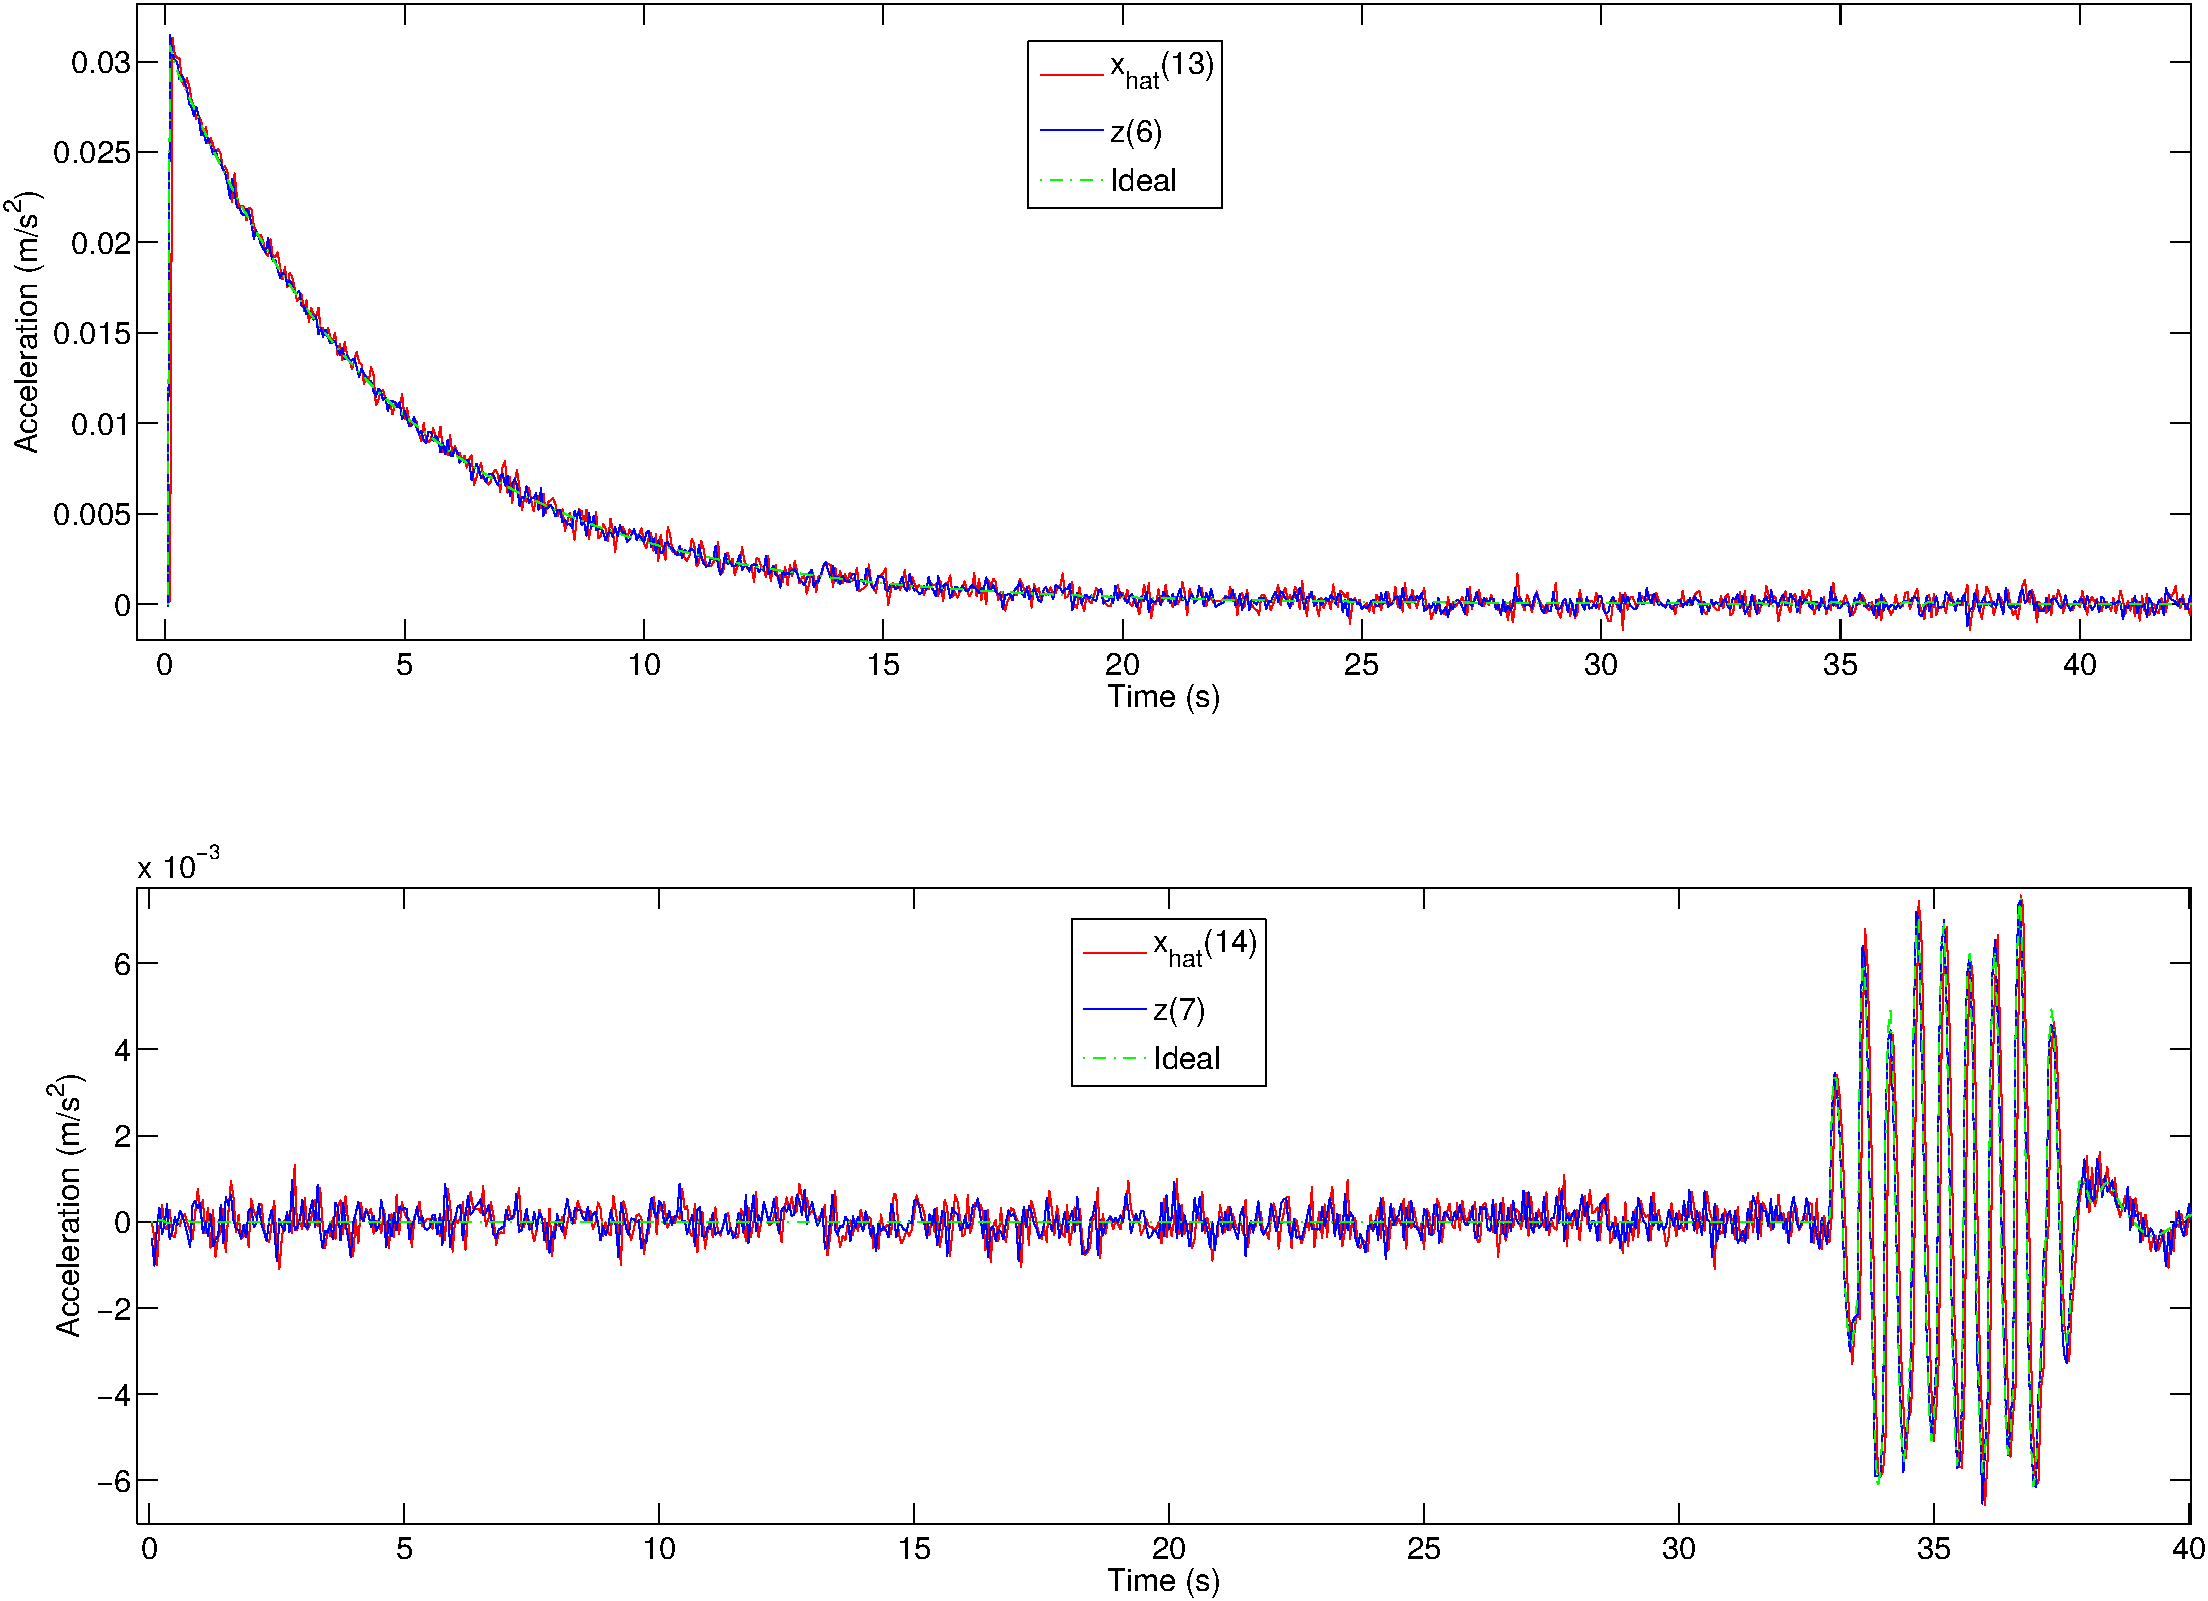
\includegraphics[width=0.9\textwidth]{../../code/matlab/accel0,00001}
%    \caption{\scriptsize Tuned acceleration with the ending Q matrix.}
%    \label{fig:acceltuning}
%  \end{figure}
%\end{frame}
%
%\begin{frame}{Simulation and Verificaiton}{Kalman Filter}
%Velocity tuning
%  \begin{figure}
%    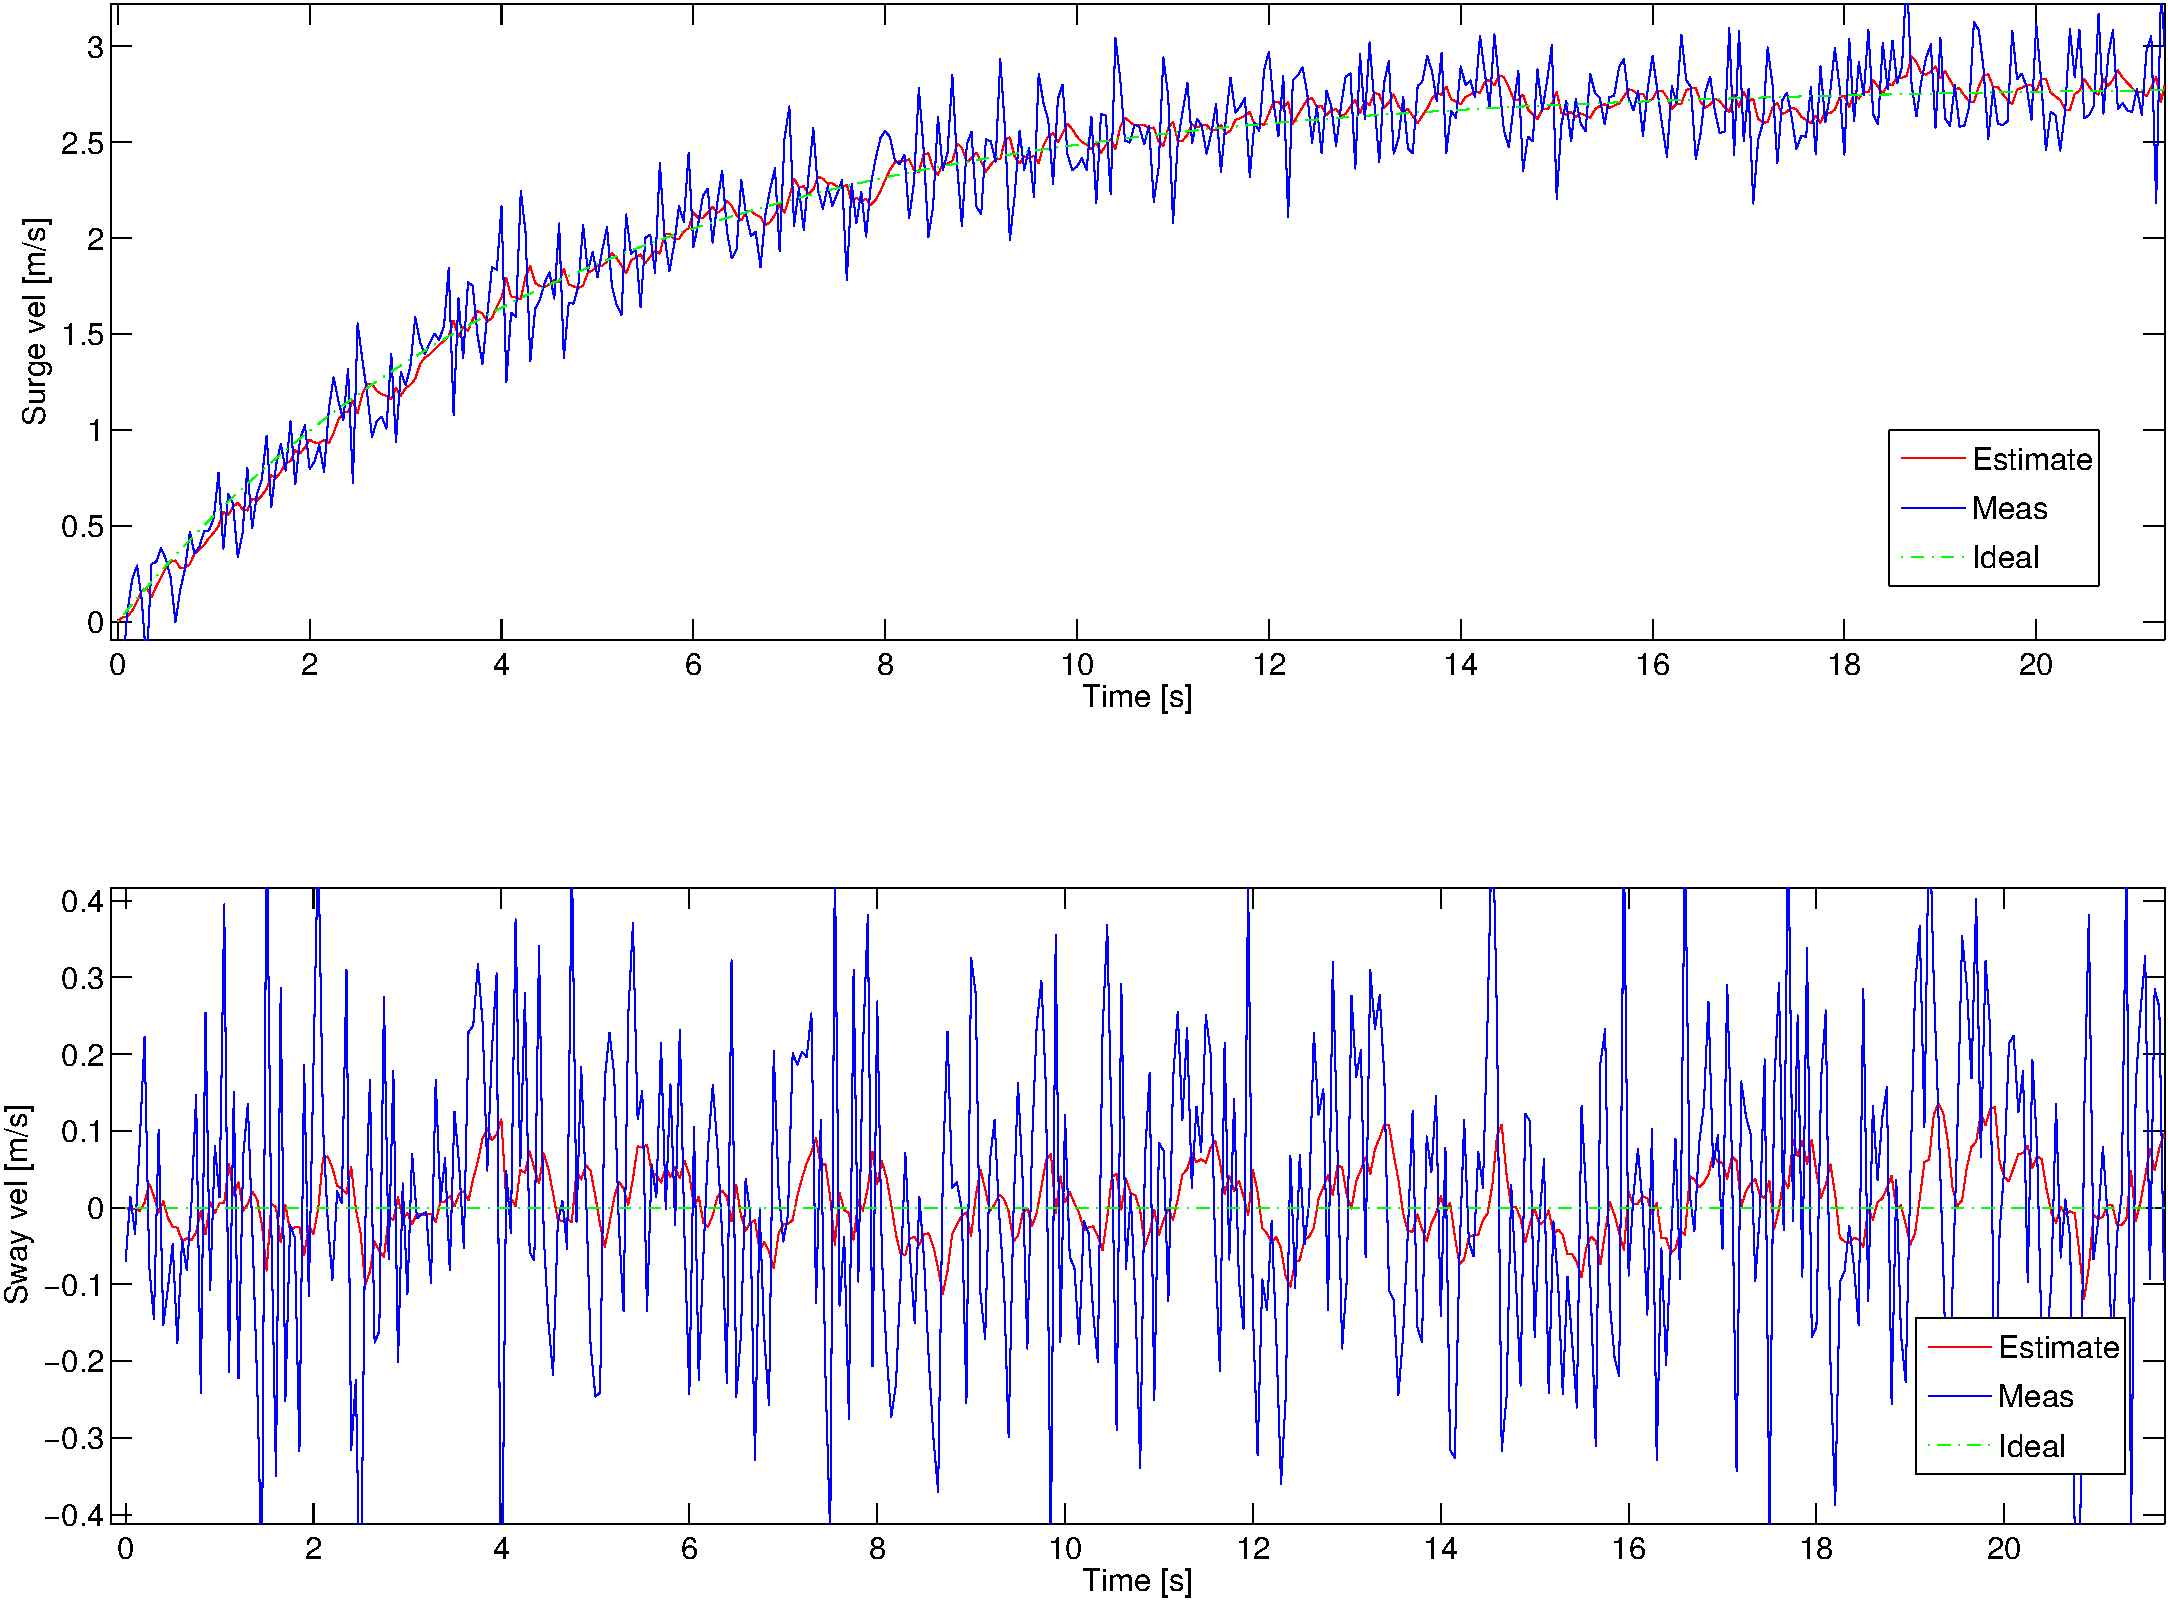
\includegraphics[width=0.9\textwidth]{../../code/matlab/uv0,00001}
%    \caption{\scriptsize Tuned velocity with the ending Q matrix.}
%    \label{fig:uvtuning}
%  \end{figure}
%\end{frame}
%
%\begin{frame}{Simulation and Verificaiton}{Kalman Filter}
%  \begin{figure}
%    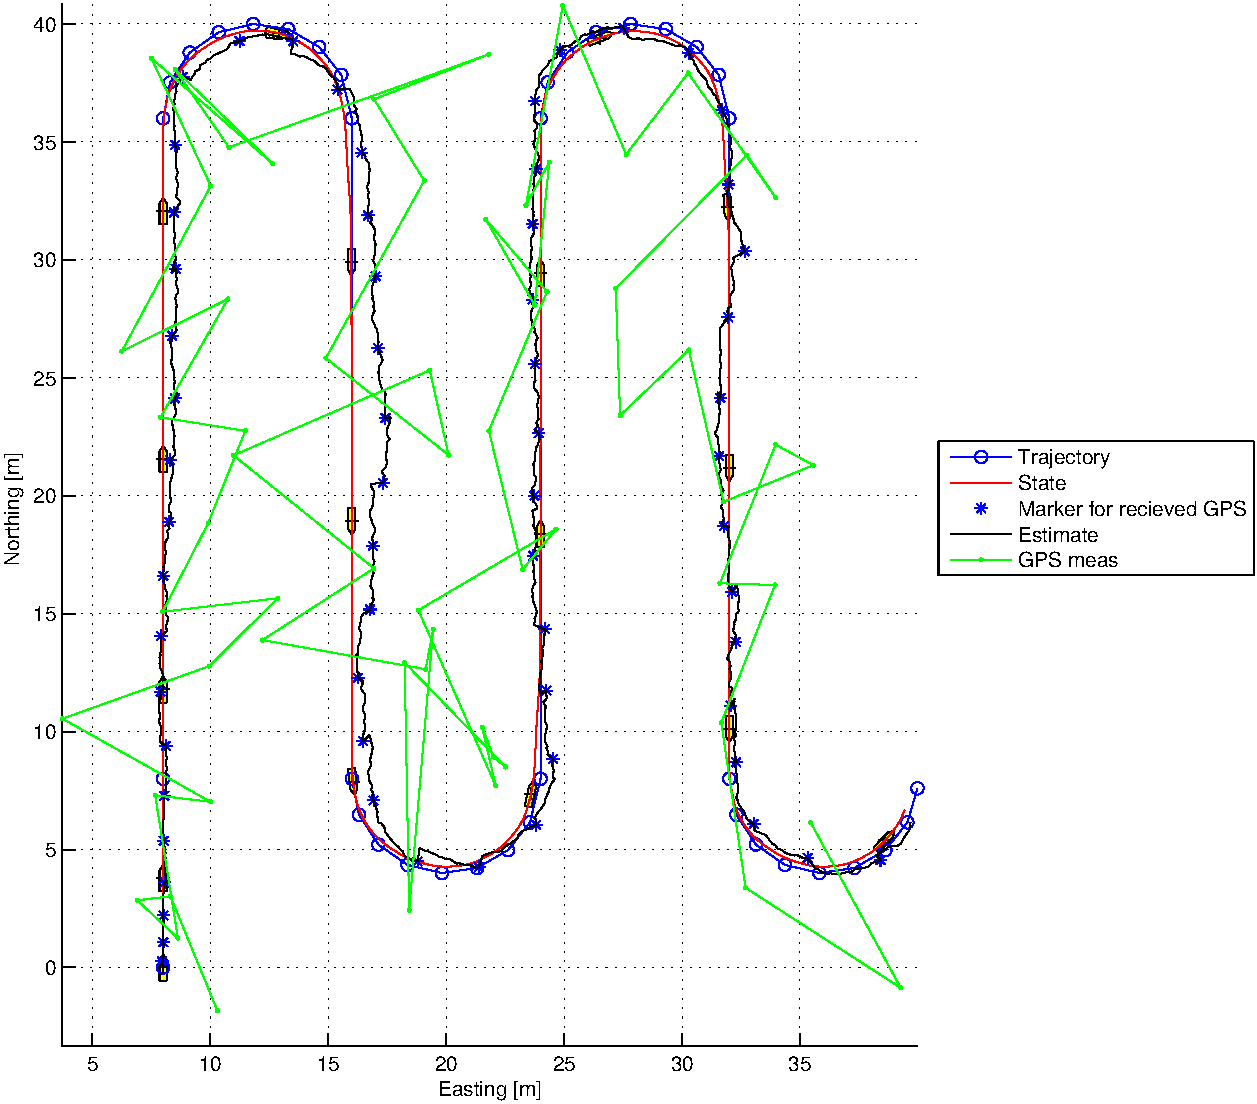
\includegraphics[width=0.65\textwidth]{../../code/matlab/q0,001}
%    \caption{\scriptsize Position tuning, $Q_{1:2,1:2}$ = 0.001. The mean/max error is 0.53m/1.67m.}
%    \label{fig:q0.001}
%  \end{figure}
%\end{frame}

\begin{frame}{Simulation and Verificaiton}{Kalman Filter}
  \begin{figure}
    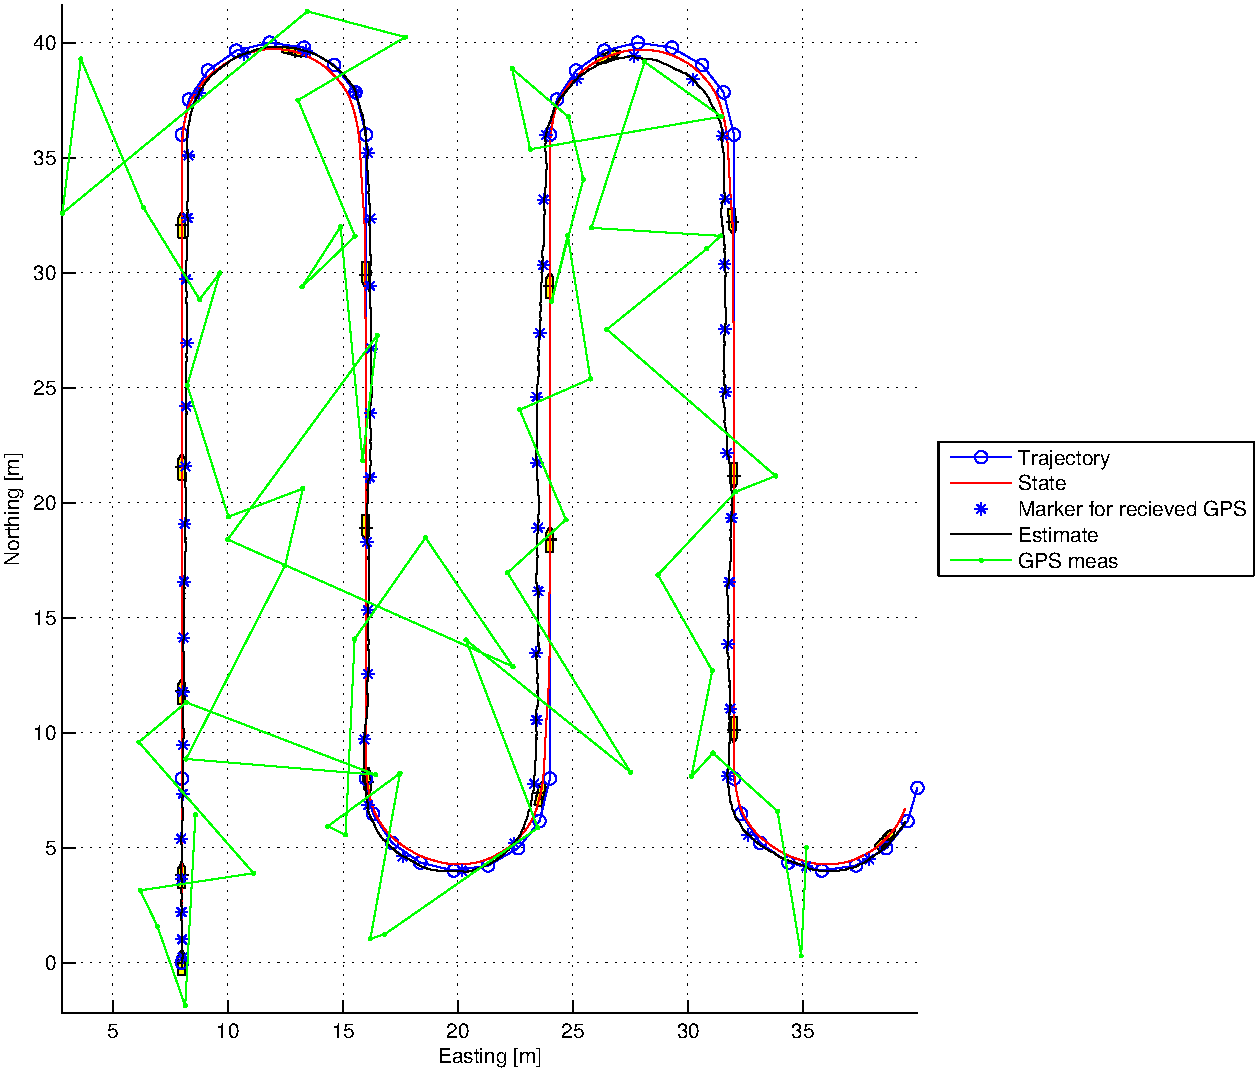
\includegraphics[width=0.65\textwidth]{../../code/matlab/q0,0001}
    \caption{\scriptsize Position tuning, $Q_{1:2,1:2}$ = 0.0001. The mean/max error is 0.32m/0.87m.}
    \label{fig:q0.0001}
  \end{figure}
\end{frame}

%\begin{frame}{Simulation and Verificaiton}{Kalman Filter}
%  \begin{figure}
%    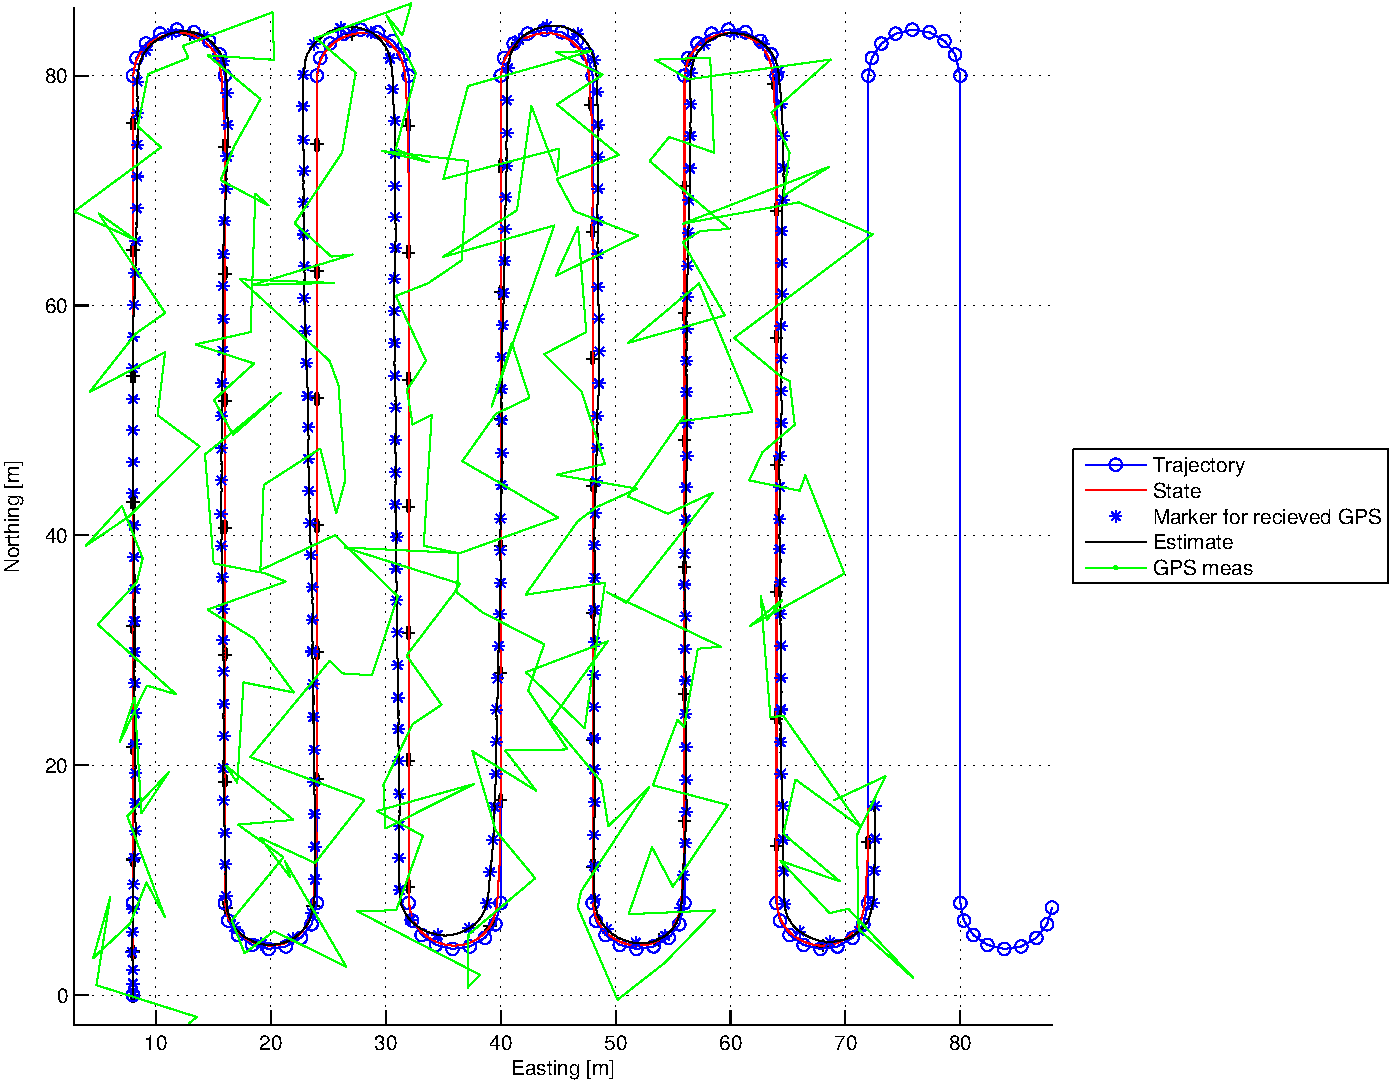
\includegraphics[width=0.65\textwidth]{../../code/matlab/q0,00001}
%    \caption{\scriptsize Position tuning, $Q_{1:2,1:2}$ = 0.00001. The mean/max error is 0.19m/0.44m.}
%    \label{fig:q0.00001}
%  \end{figure}
%\end{frame}

%\begin{frame}{Simulation and Verificaiton}{Comparision between KF and AHRS}
%  \begin{figure}
%    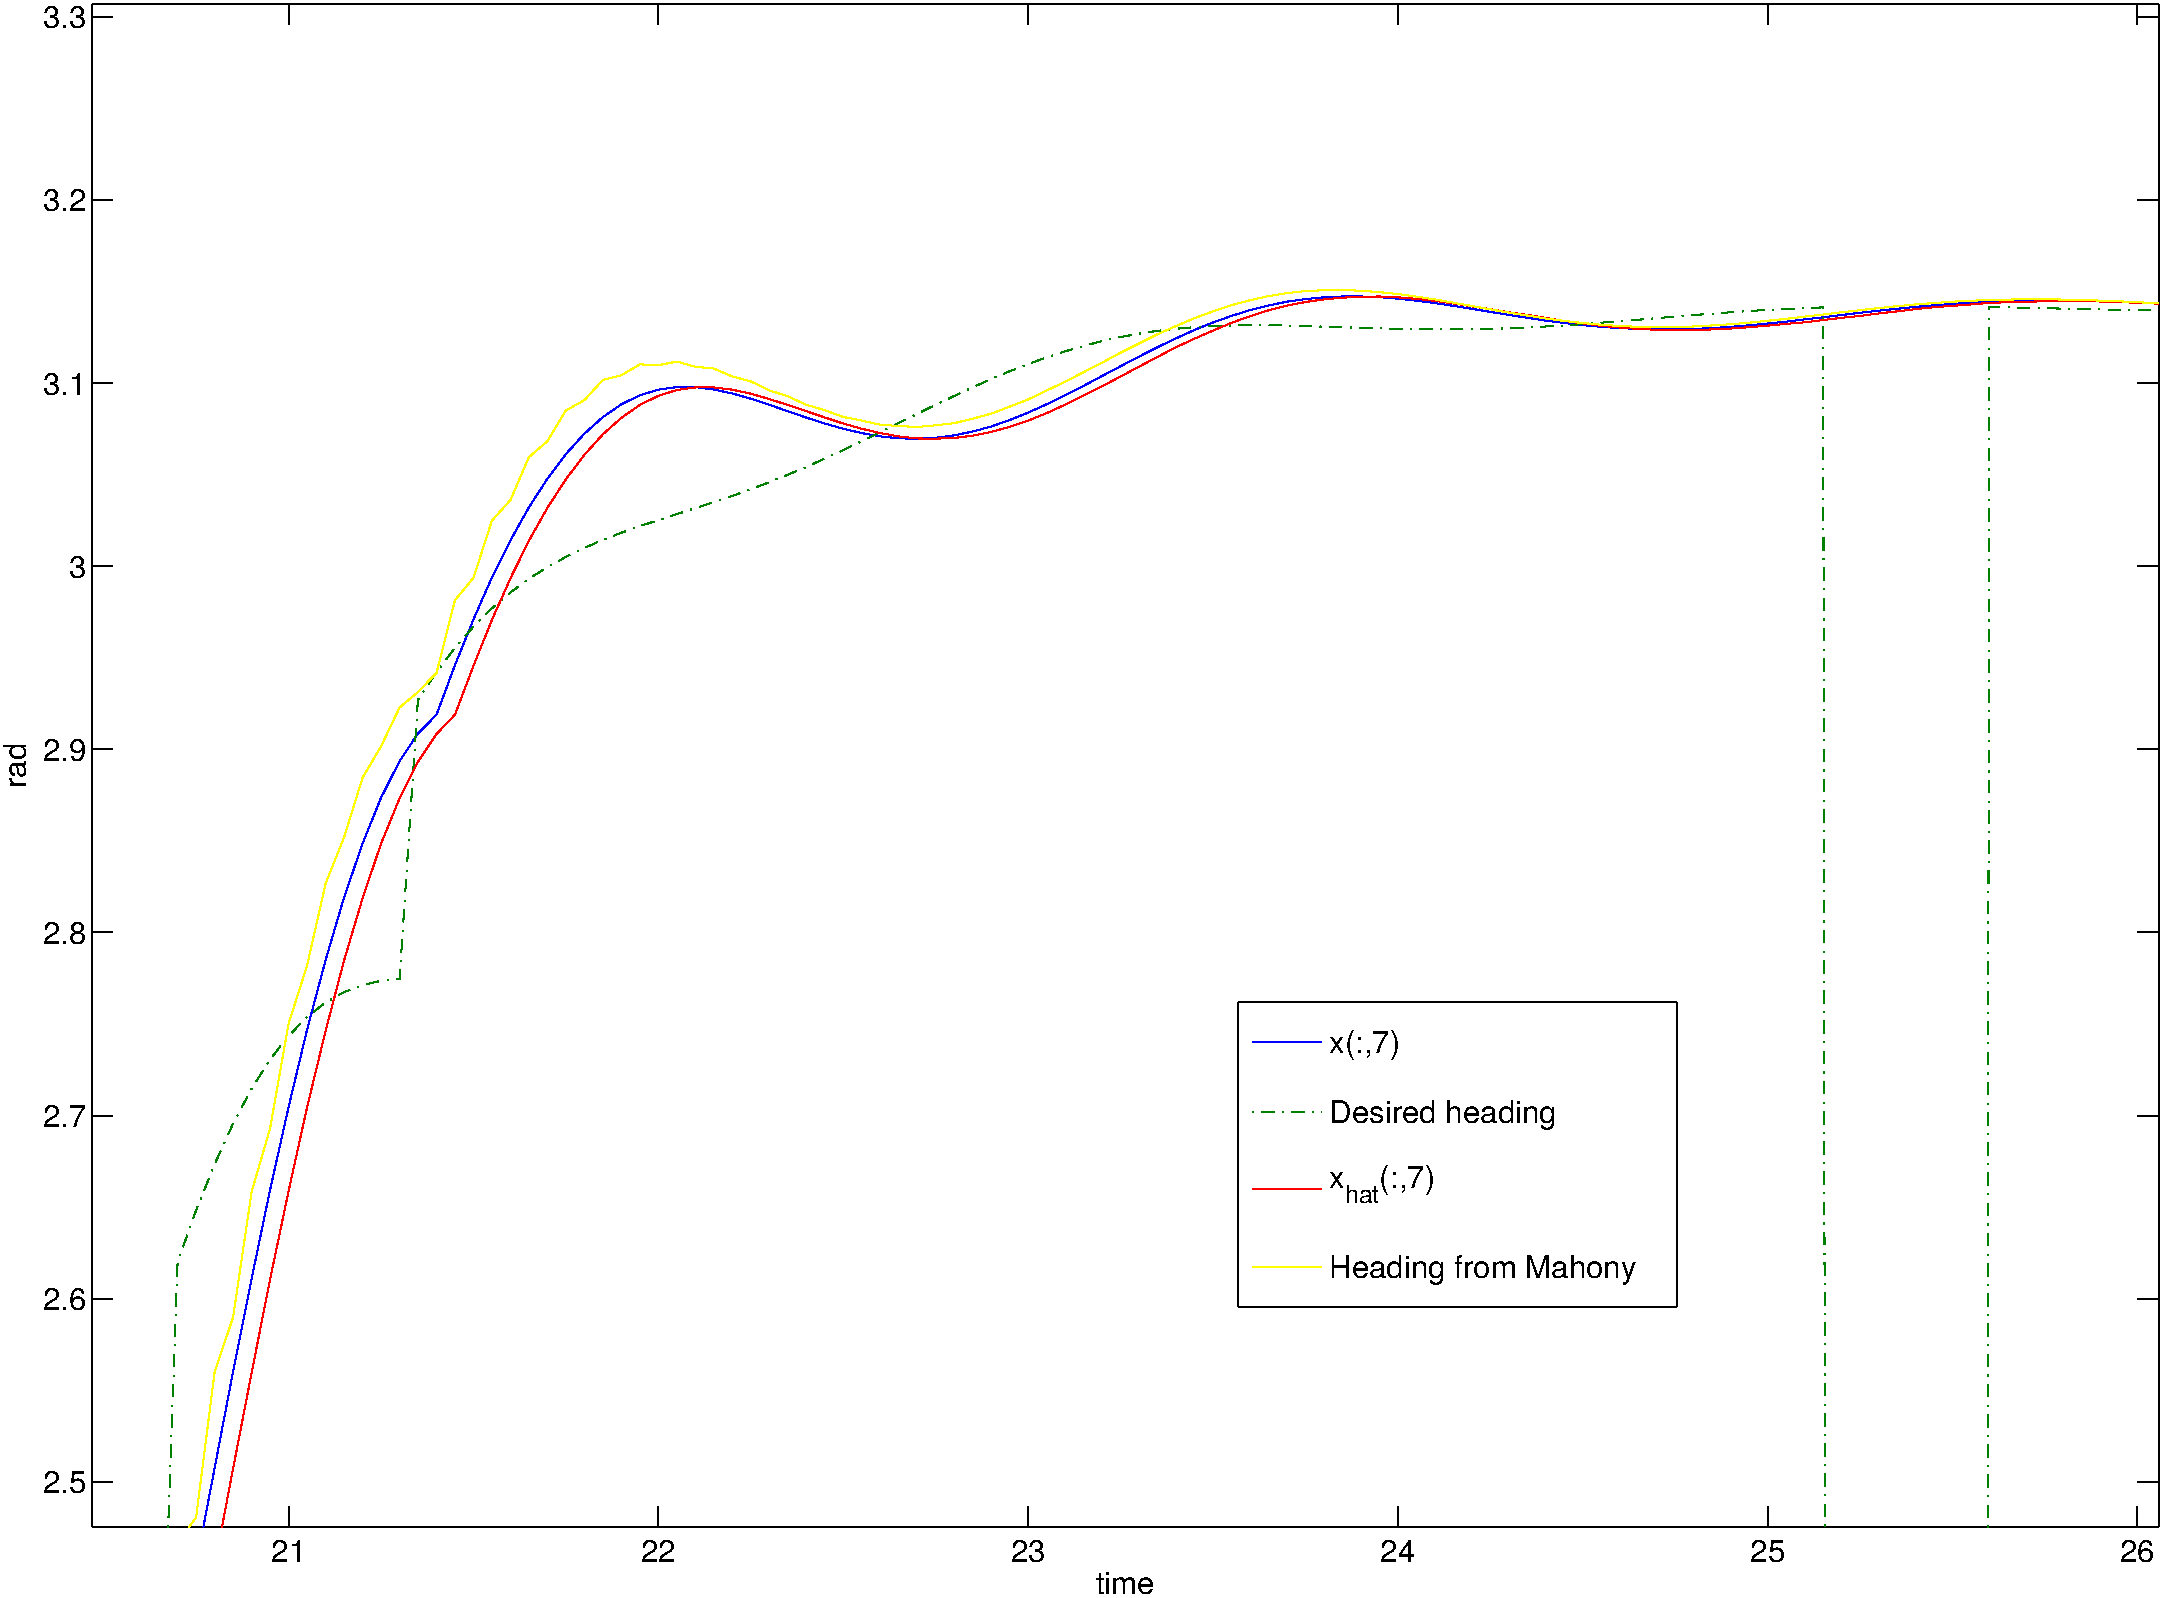
\includegraphics[width=0.9\textwidth]{../../code/matlab/mahonyvskf}
%    \caption{\scriptsize Heading estimation by the KF and the Mahony filters.}
%    \label{fig:mavskf}
%  \end{figure}
%\end{frame}

\begin{frame}{Simulation and Verification}{ROS demo With single ship}
<Video of Single Ship in ROS>
\texttt{aauship-ros-rviz-simulation-demo.ogv}
\end{frame}

\begin{frame}{Simulation and Verification}{Data from sea trial}
    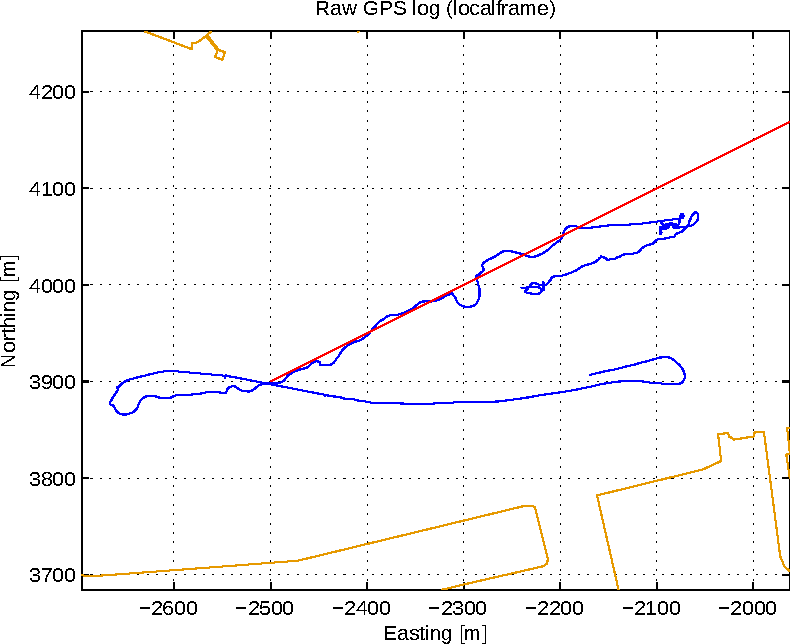
\includegraphics[width=0.95\textwidth]{img/test1}
\end{frame}

%\begin{frame}{Simulation and Verificaiton}{Loose Ends}
%\begin{itemize}
%  \item Interface between the \texttt{/lli\_input} topic is not compatible with the LLI
%  \item Optionally extend the KF with the second GPS and use dilution of precision to modify the observational covariance matrix
%  \item Thrust allocation needs testing and implementation
%  \item The GPS data needs to be handled in ROS
%  \item Lab test with the hardware in the loop to test that interfaces work
%  \item Sea-trail needed to verify that it all works
%\end{itemize}
%\end{frame}

%%%%%%%%%%%%%%%%%
%\section{Schedule}
%\begin{frame}{Schedule}{2nd Half Goals}
%Design and implementation of formation control on the platforms
%  \begin{itemize}
%  \item Assembly of two other boats, same as the one we have
%  \item Analyse different formation control strategies in more detail
%  \item Determination of practical group coordination (initialisation task)
%  \item Implementation of leader-follower formation control (tracking task)
%  \item Formation control is according to a given path of interest
%  \item Extend simulation model with environmental disturbances
%  \item Agent-agent avoidance, and maybe other objects too
%  \end{itemize}
%\end{frame}
\section{Formation Strategies}
\begin{frame}{Formation Strategies}{Which to choose}
Several different strategies that have been considered
  \begin{itemize}
    \item Leader follower
    \begin{itemize}
      \item Duckling/Echelon/FRP
    \end{itemize}
    \item Individual paths
    \begin{itemize}
      \item Potential fields
    \end{itemize}
   \end{itemize}
\end{frame}

\begin{frame}{Formation Strategies}{Why these}
Estimate of performance in categories
\begin{itemize}
  \item Communication
  \item Control architecture
  \item Obstacle avoidance
  \item Transients
  \item Scalability
  \item Failure
\end{itemize}
\begin{figure}
    {\tiny \includesvg[width=\textwidth]{potentialfield_block}}
    \caption{\scriptsize Structure of the signals in the potential field}
  \end{figure}
\end{frame}

\begin{frame}{Formation Strategies}{The chosen}
The chosen strategy is:
\begin{itemize}
  \item Potential field
\end{itemize}
Other strategies have briefly been analysed, like:
\begin{itemize}
\item Duckling formation
\item Echelon formation
\end{itemize}
\end{frame}

\begin{frame}{Leader Follower}{Echelon formation}
  \begin{figure}
    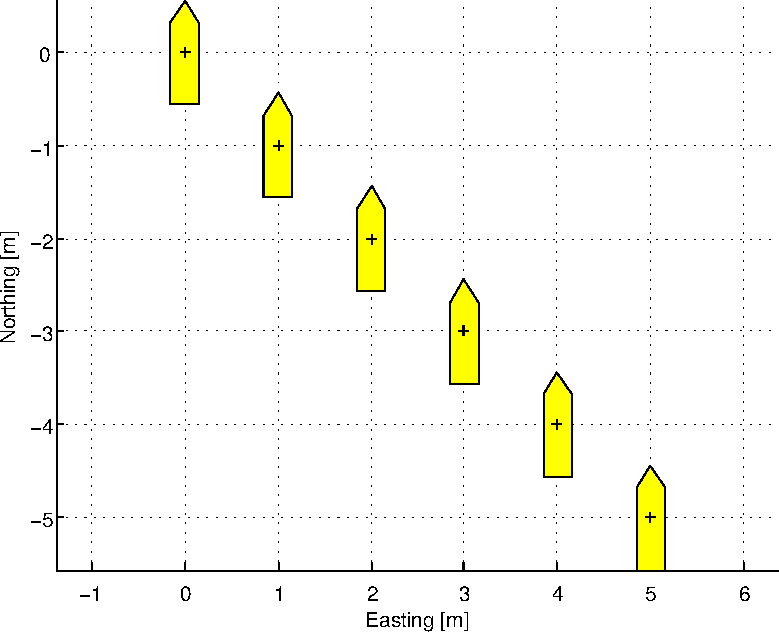
\includegraphics[width=0.65\textwidth]{img/echelon}
    \caption{The leader follow approach as echelon form}
    \label{fig:echelon}
  \end{figure}
\end{frame}

\section{Potential Field}

\begin{frame}{Potential field}{Single ship application}
  \begin{figure}
    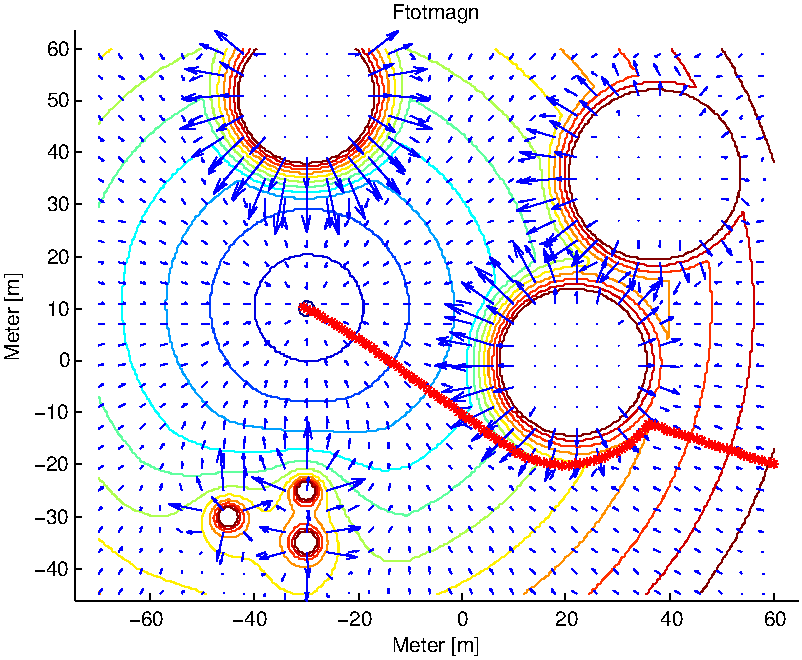
\includegraphics[width=0.65\textwidth]{img/ftotmagnfigpdf}
    \caption{Potential field for a single ship}
    \label{fig:potsingleship}
  \end{figure}
\end{frame}

\begin{frame}{Potential Field}{Formation with potential field}
<Simulation video of the potential field in action>
\texttt{media/v-formation-animation.ogv}
\end{frame}

\begin{frame}{Potential Field}{The implementation}
Central algorithms before:
\begin{itemize}
\item wp\_gen
\item pathgen(potfield)
\end{itemize}
Algorithm after:
\begin{itemize}
\item potfield
\end{itemize}
\end{frame}

\begin{frame}{Potential Field}{Validation and error plots}
  \begin{figure}
    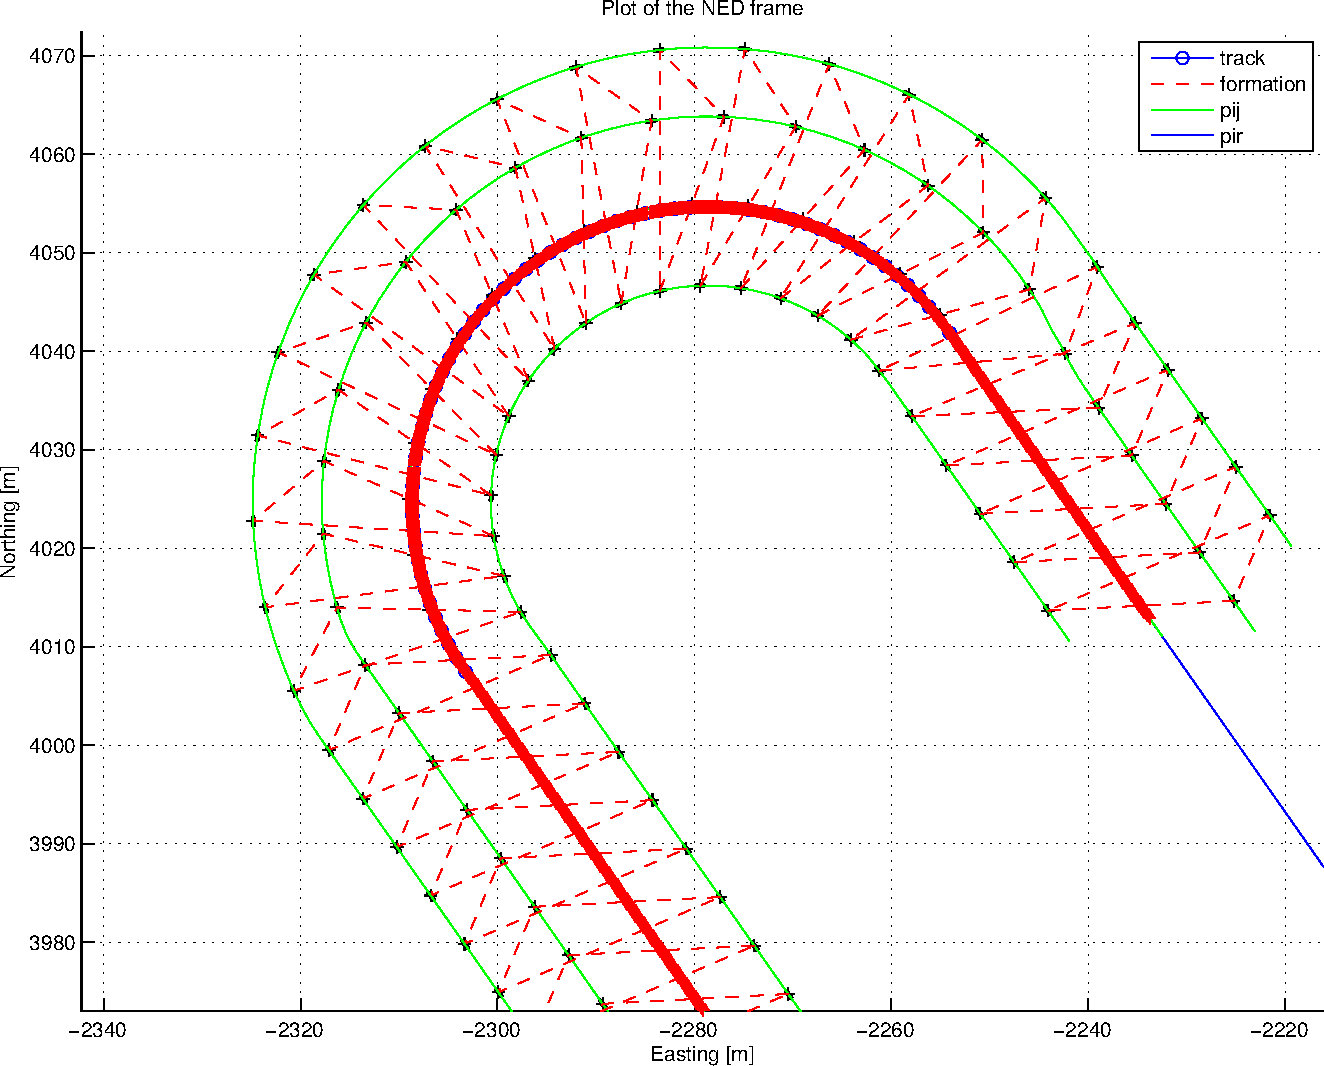
\includegraphics[width=0.85\textwidth]{img/pdftotalligeplussving}
    \caption{Plot of tracking phase around a turn}
  \end{figure}
\end{frame}

\begin{frame}{Potential Field}{Validation and error plots}
  \begin{figure}
    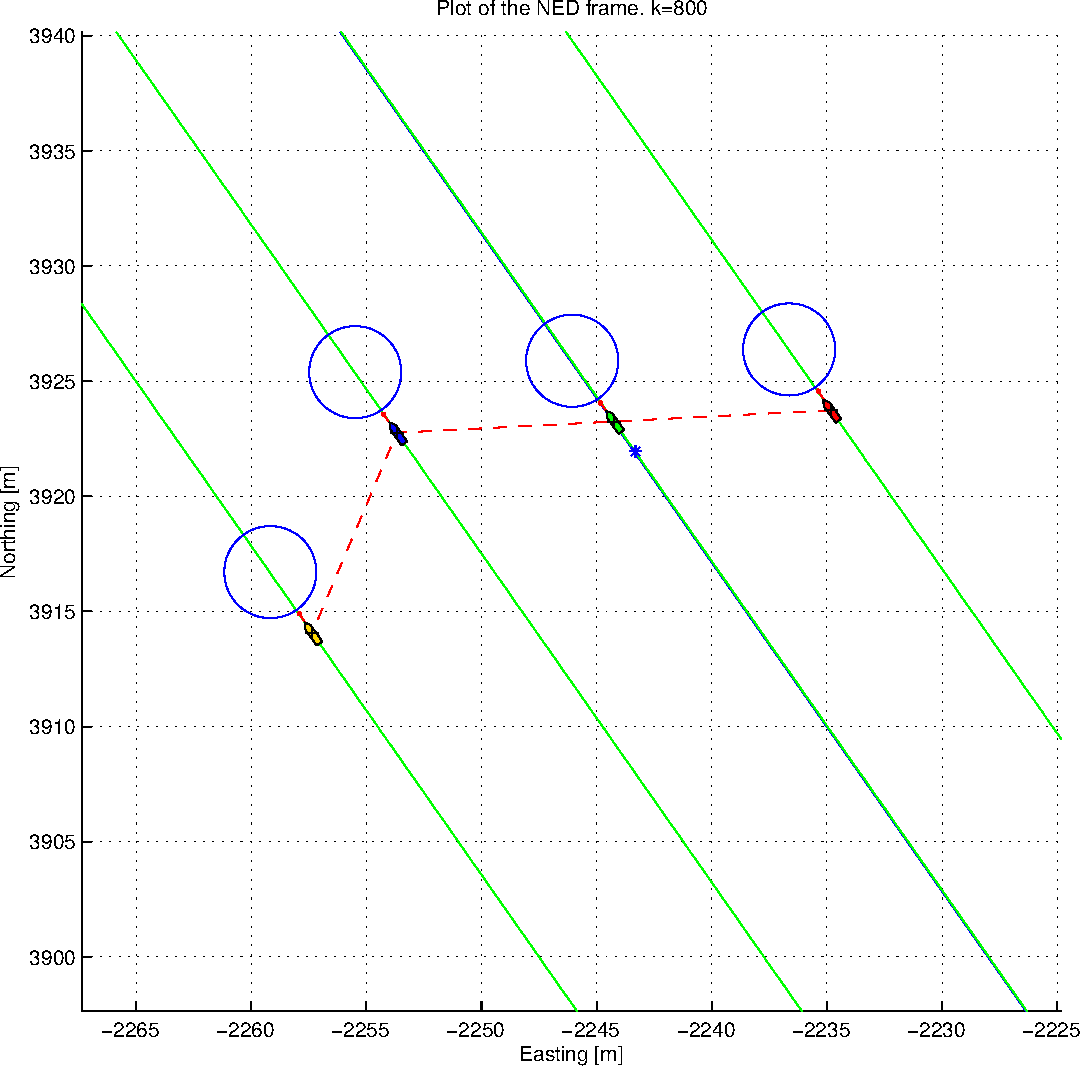
\includegraphics[width=0.7\textwidth]{img/pdfligestykke}
    \caption{Plot of tracking phase on straight line segment}
  \end{figure}
\end{frame}

\begin{frame}{Potential Field}{Validation and error plots}
  \begin{figure}
    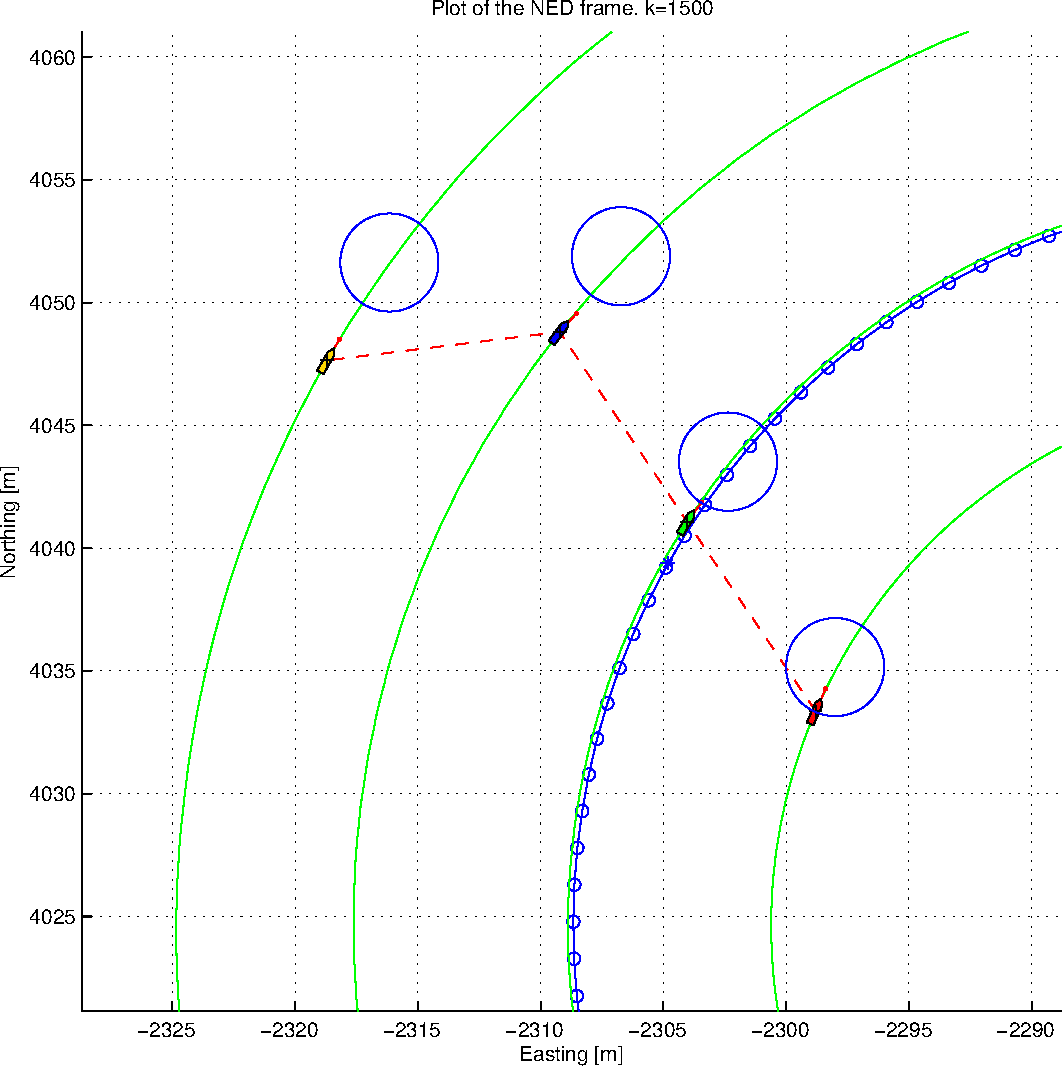
\includegraphics[width=0.7\textwidth]{img/pdfsvingstykke}
    \caption{Plot of tracking phase in right turn}
  \end{figure}
\end{frame}

\begin{frame}{Potential Field}{Validation and error plots}
  \begin{figure}
    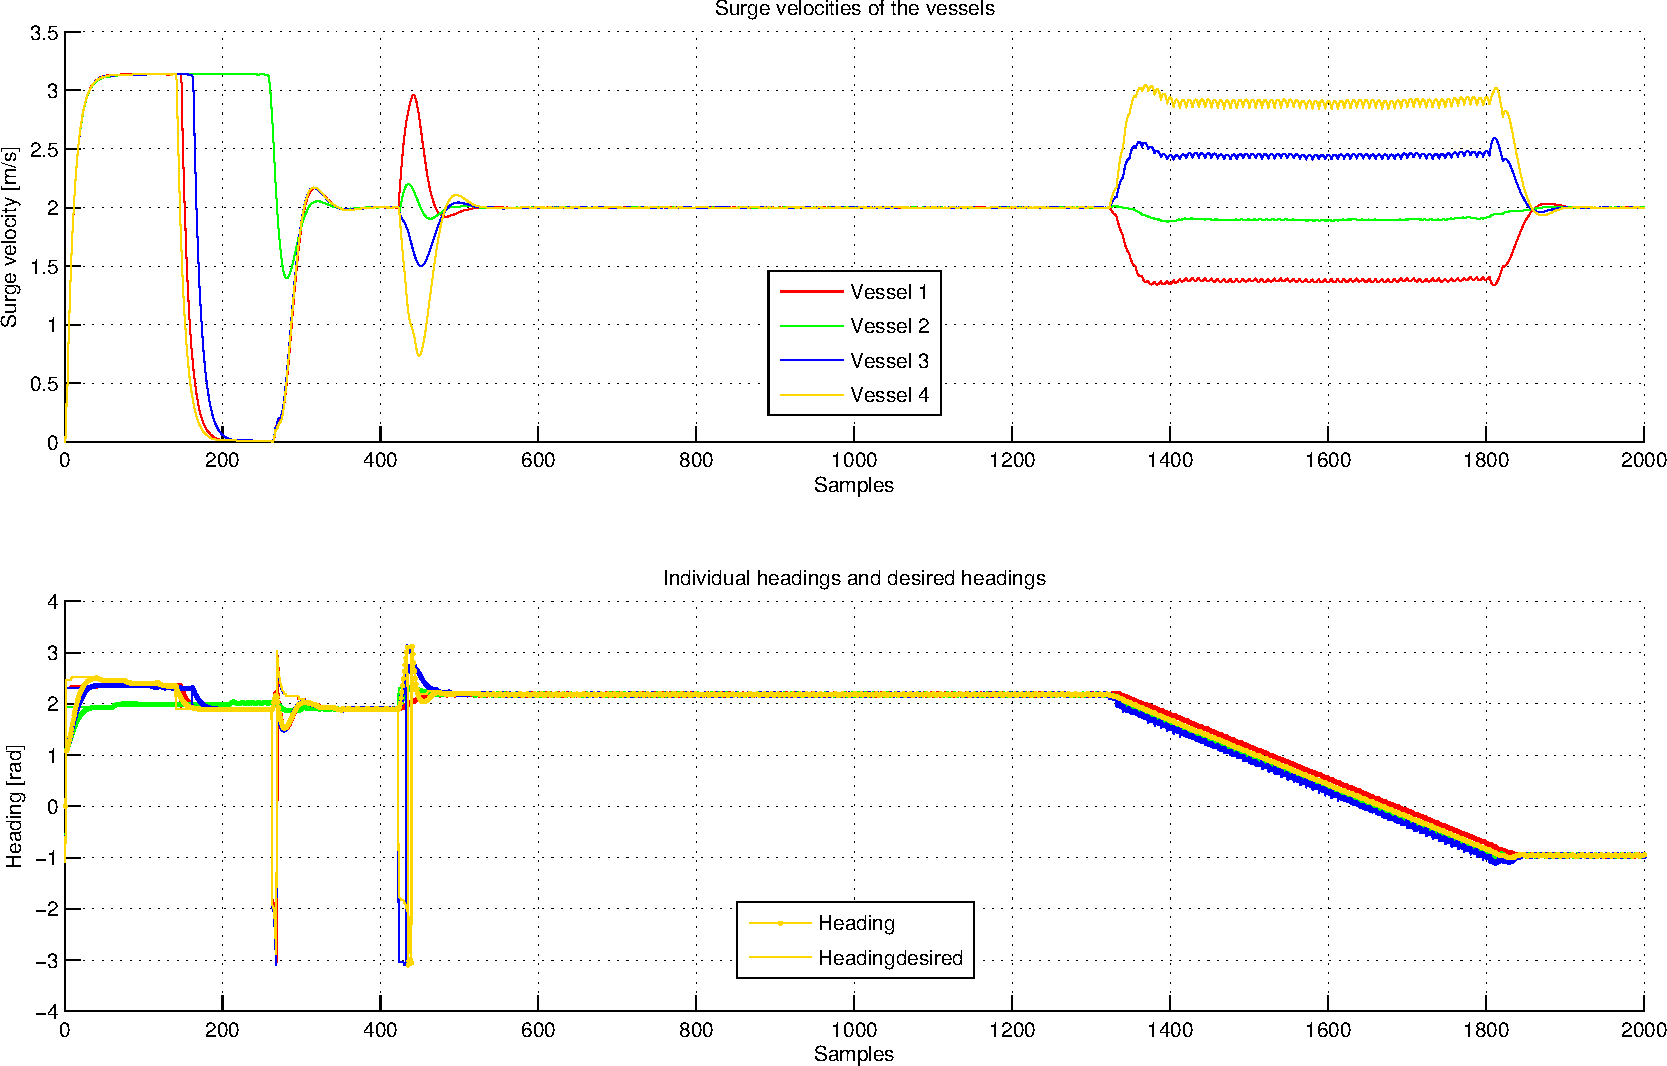
\includegraphics[width=\textwidth]{img/pdfveloghead}
    \caption{Plot of velocities and heading of individual vessels}
  \end{figure}
\end{frame}

\begin{frame}{Potential Field}{Validation and error plots}
  \begin{figure}
    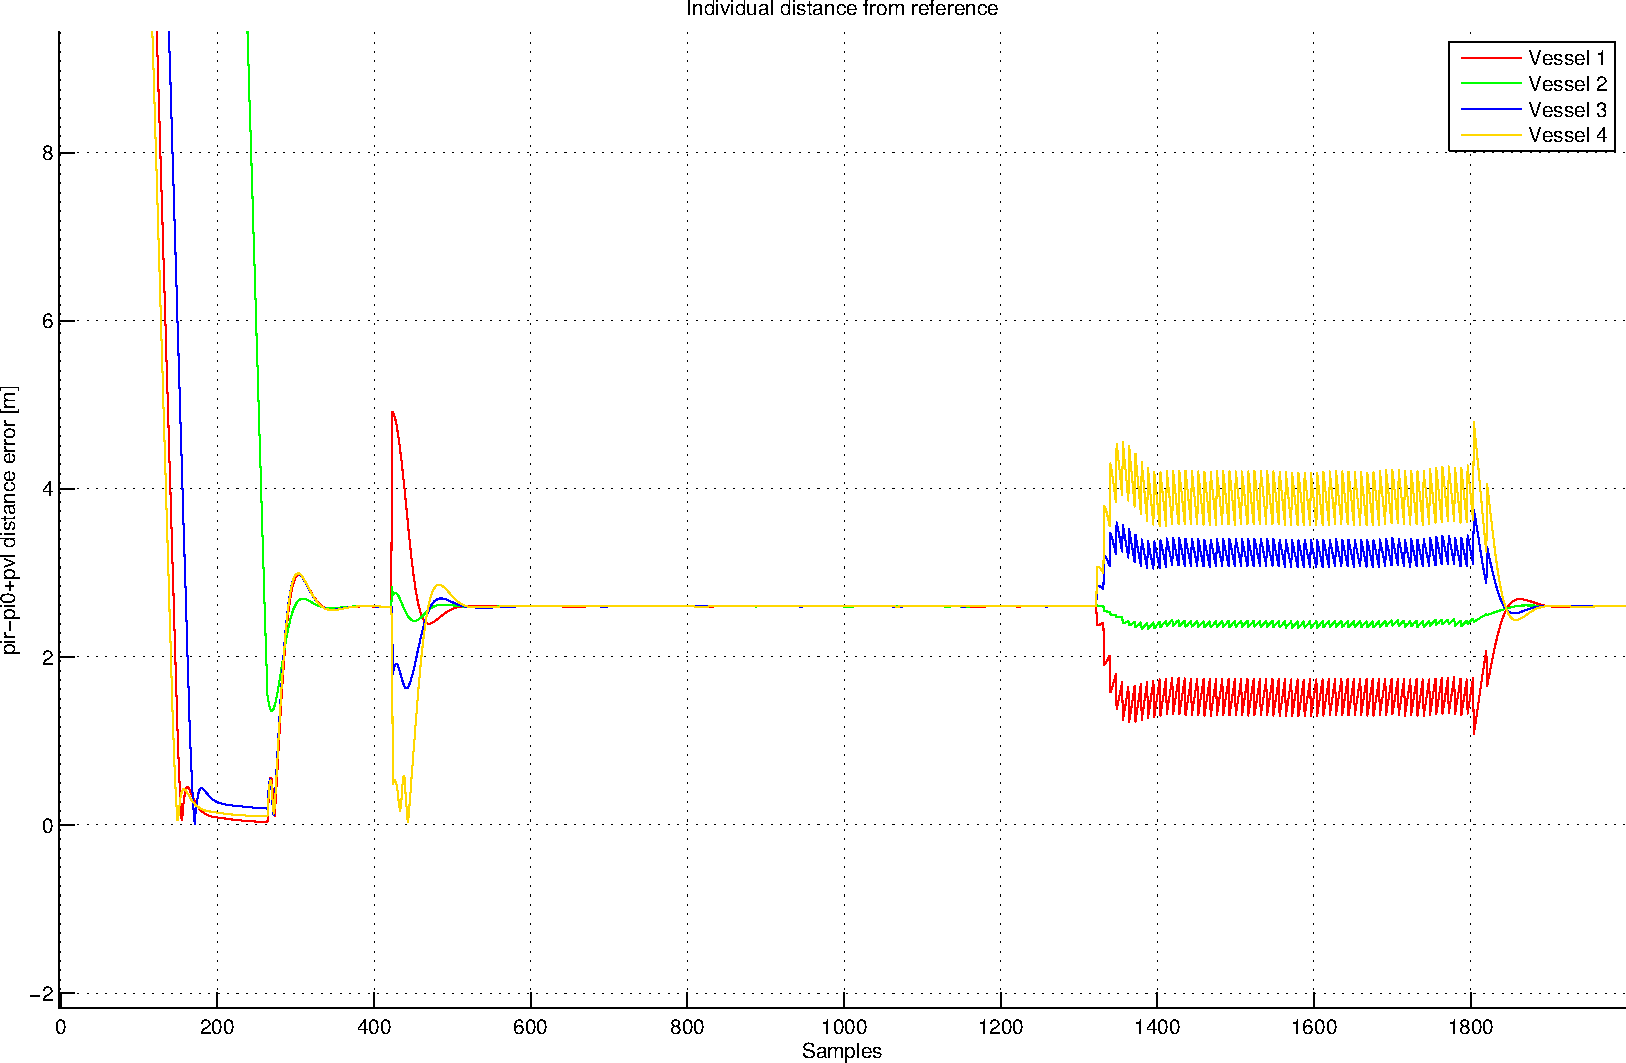
\includegraphics[width=\textwidth]{img/pdfdistfromref}
    \caption{Plot of individual distances to the reference}
  \end{figure}
\end{frame}

\begin{frame}{Potential Field}{Performance dependencies}
  \begin{figure}
    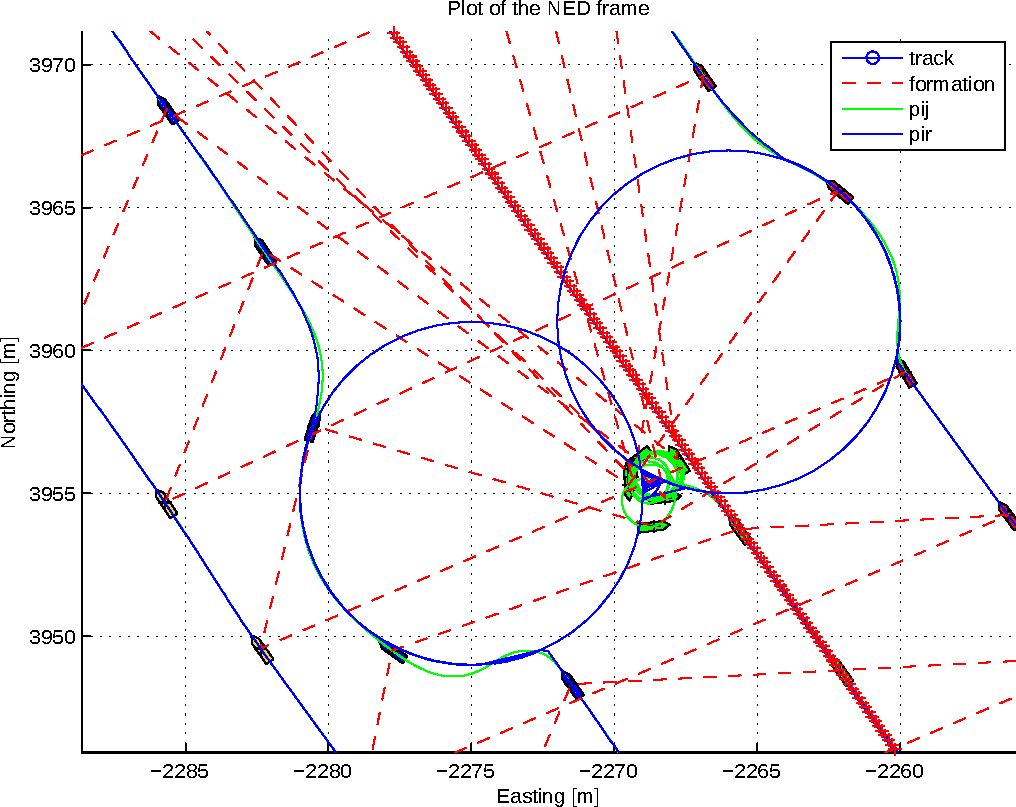
\includegraphics[width=0.95\textwidth]{img/wp_gen_ass_fail}
    \caption{Minimum magnitude method}
  \end{figure}
\end{frame}

\begin{frame}{Potential Field}{Performance dependencies}
  \begin{figure}
    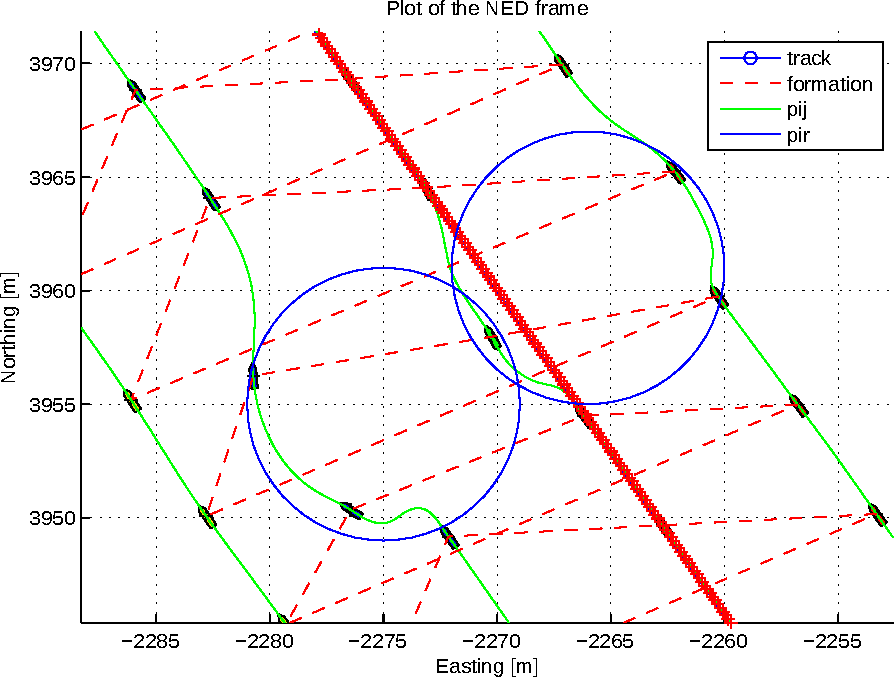
\includegraphics[width=\textwidth]{img/wp_gen_ass_vector}
    \caption{Force vector method}
  \end{figure}
\end{frame}

\section{Conclusion}

\begin{frame}{Conclusion}{Status}
\begin{itemize}
  \item Hardware upgrade
  \item Upgrade to ROS
  \item Model of vessel
  \item Test of vessel
  \item Analysed strategies and framework
  \item Simulation of chosen strategy
  \begin{itemize}
  \item Initialisation task
  \item Tracking task
  \item Avoidance
  \end{itemize}
\end{itemize}
\end{frame} 

\begin{frame}{Further Work}{What can be done in other ways}
\begin{itemize}
\item Implementation of the formation control strategy in ROS
\item Communication topology
\item Other controllers
\item Extend model
\item Fault detection and handling
\item Building the fleet
\end{itemize}
\end{frame}

{
\setbeamertemplate{background canvas}{\centering\includegraphics[height=\paperheight,keepaspectratio]{{img/aauship}}}
\begin{frame}[plain]{}\end{frame}}

\end{document}
